\section{Milestone principali}
\label{sec:milestone_principali}
\subsection{RTB: Requirements and Technology Baseline}
Si tratta della prima revisione che viene realizzata per valutare lo stato di avanzamento de lavoro e la qualità con cui è stato svolto.
Raggiunta la data stabilita dal gruppo per l'\glossario{RTB} dovranno essere realizzati i seguenti prodotti:

\begin{itemize}
\item Analisi dei Requisiti;
\item Piano di Progetto;
\item Piano di Qualifica;
\item Proof of Concept (\glossario{PoC}).
\end{itemize}

\subsubsection{Preventivo}
Il gruppo considera le seguenti date per lo sviluppo dell'\glossario{RTB}:
\begin{itemize}
    \item Data di inizio: 12 Novembre 2024;
    \item Data di fine: 10 Febbraio 2025.
\end{itemize}
L'analisi realizzata ha permesso di stabilire i compiti per ogni ruolo fino alla data dell'\glossario{RTB}:
\begin{itemize}
\item Responsabile: dovrà organizzare ogni settimana le attività da svolgere, il prospetto è di utilizzare il 45\% delle ore totali assegnate;

\item Amministratore: dovrà organizzare gli strumenti necessari allo svolgimento delle attività per l'\glossario{RTB}, mantenendo aggiornato il documento delle Norme di progetto.
Il prospetto è di utilizzare il 59\% delle ore totali assegnate;

\item Analista: per questo ruolo ci si aspetta di utilizzare quasi interamente le ore assegnate (vengono tenute ore a disposizione che facciano da cuscinetto in caso di necessità), avrà il compito di realizzare l'analisi dei requisiti e di effettuare la stesura del documento.
Il prospetto è di utilizzare il 90\% delle ore totali assegnate;

\item Progettista: ci si aspetta non vengano utilizzate le sue ore assegnate in quanto, siccome il \glossario{PoC} consiste in un artefatto usa e getta, non verrà realizzata progettazione del software fino alla data dell'\glossario{RTB}.
Il prospetto è di utilizzare lo 0\% delle ore totali assegnate;

\item Programmatore: avrà il compito di realizzare il \glossario{PoC} per dimostrare la fattibilità del progetto e la capacità del gruppo di realizzarlo.
Il prospetto è di utilizzare il 27\% delle ore totali assegnate;

\item Verificatore: avrà il compito di effettuare la verifica dei documenti realizzati e dei requisiti analizzati dall'analista, non ci si aspetta verifica di codice per il \glossario{PoC}, non necessaria in quanto è un artefatto usa e getta.
Il prospetto è di utilizzare il 30\% delle ore totali assegnate.
\end{itemize}
Nella seguente tabella viene riportata una stima delle ore e i costi per ruolo preventivati fino all'\glossario{RTB}:
\begin{table}[H]
    \centering
    \resizebox{\textwidth}{!}{
    \begin{tabular}{| l | l | l | l |}
        \hline
            \textbf{Ruolo} &  
            \textbf{Ore per ruolo} & 
            \textbf{Costo orario} &
            \textbf{Costo totale} \\
        \hline
        \hline
            Responsabile & 20 & 30€ & 600€ \\
        \hline
            Amministratore & 32 & 20€ & 640€ \\
        \hline 
            Analista & 70 & 25€ & 1750€ \\
        \hline 
            Progettista & 0 & 25€ & 0€ \\
        \hline 
            Programmatore & 40 & 15€ & 600€ \\
        \hline 
            Verificatore & 45 & 15€ & 675€ \\
        \hline 
            \textbf{Totale} & \textbf{207} & \textbf{N/A} & \textbf{4265€} \\ 
        \hline  
    \end{tabular}}
    \caption{Ripartizione ore e costi fino RTB.}
    \label{tab:stima_costi_RTB} 
\end{table}

Di seguito viene mostrato un diagramma a torta in cui viene indicata la ripartizione dei ruoli in percentuale rispetto le ore totali preventivate per la realizzazione dei prodotti da consegnare entro la data stabilita per l'\glossario{RTB}.

\begin{figure}[H]
    \centering
    \begin{tikzpicture}
        \pie{9.66/Responsabile, 15.46/Amministratore, 33.82/Analista, 19.32/Programmatore, 21.74/Verificatore}
    \end{tikzpicture}
    \caption{Ripartizione ore e ruoli fino a \glossario{RTB}.}
    \label{fig:pie_ruoli_RTB}
\end{figure}

\subsubsection{Consuntivo}
Le date per lo sviluppo dell'\glossario{RTB} sono state:
\begin{itemize}
    \item Data di inizio: 12 Novembre 2024;
    \item Data di fine: 20 Marzo 2025.
\end{itemize}
Le ore per ruolo utilizzate rispetto al totale e le considerazioni sono indicate nella seguente lista:
\begin{itemize}
    \item Responsabile: sono state utilizzate il 46\% delle ore.
    Quindi preventivo per il ruolo è stato ecceduto per una soglia accettabile;

    \item Amministratore: sono state utilizzate il 59\% delle ore.
    Quindi il preventivo per il ruolo è risultato corretto;
    
    
    \item Analista: sono state utilizzate il 95\% delle ore per questo ruolo, quindi il preventivo è risultato troppo stretto.
    Dato che l'analisi dei requisiti è stata eseguita in modo approfondito le ore rimaste per questo ruolo verranno riassegnate;

    \item Progettista: sono state utilizzate il 0\% delle ore per questo ruolo, infatti come previsto il gruppo ha sviluppato il \glossario{PoC} come un artefatto usa e getta;
    
    \item Programmatore: sono state utilizzate il 20\% delle ore per questo ruolo.
    In particolare il gruppo ha notato che le ore preventivate per il ruolo di Programmatore per l'intero progetto sono eccessive e quindi verranno riassegnate;
    
    \item Verificatore: sono state utilizzate il 40\% delle ore per questo ruolo.
    Dal consuntivo per questo ruolo il gruppo ha 
\end{itemize}
Nella \hyperref[tab:consuntivo_RTB]{Tabella \ref{tab:consuntivo_RTB}} viene riportato il consuntivo delle ore e dei costi per ruolo sostenuti fino all'\glossario{RTB}:
\begin{table}[H]
    \centering
    \resizebox{\textwidth}{!}{
    \begin{tabular}{| l | l | l | l |}
        \hline
            \textbf{Ruolo} &  
            \textbf{Ore per ruolo} & 
            \textbf{Costo orario} &
            \textbf{Costo totale} \\
        \hline
        \hline
            Responsabile & 20.5 & 30€ & 615€ \\
        \hline
            Amministratore & 32 & 20€ & 640€ \\
        \hline 
            Analista & 74.5 & 25€ & 1862.5€ \\
        \hline 
            Progettista & 0 & 25€ & 0€ \\
        \hline 
            Programmatore & 31 & 15€ & 465€ \\
        \hline 
            Verificatore & 59.75 & 15€ & 896.25€ \\
        \hline 
            \textbf{Totale} & \textbf{217.75} & \textbf{N/A} & \textbf{4478.75€} \\ 
        \hline  
    \end{tabular}}
    \caption{Consuntivo RTB.}
    \label{tab:consuntivo_RTB} 
\end{table}
In \hyperref[fig:preventivo_consuntivo]{Figura \ref{fig:preventivo_consuntivo}} viene riportato un diagramma a blocchi che mostra il confronto tra ore preventivate e ore utilizzate per ogni ruolo:
\begin{figure}[H]
    \centering
    \resizebox{\textwidth}{!}{
    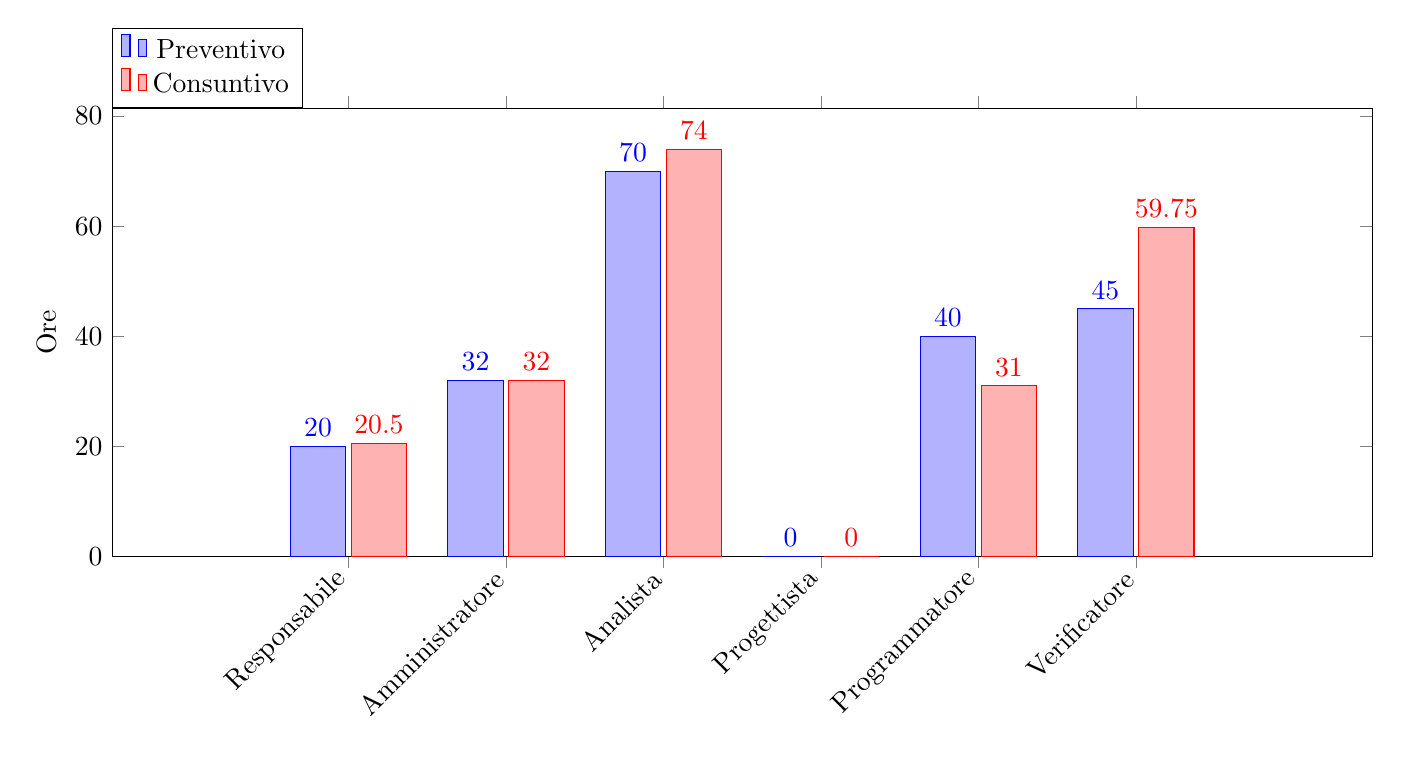
\begin{tikzpicture}
        \begin{axis}[
            ybar,
            symbolic x coords={Responsabile, Amministratore, Analista, Progettista, Programmatore, Verificatore},
            xtick=data,
            nodes near coords,
            ymin=0,
            ylabel={Ore},
            enlarge x limits=0.3,
            bar width=20pt,
            xticklabel style={rotate=45, anchor=east},
            x=2cm,
            legend style={at={(0,1)}, anchor=south west, legend columns=1}
        ]

            \addplot coordinates {(Amministratore,32) (Responsabile,20) (Analista,70) (Progettista, 0) (Programmatore, 40) (Verificatore, 45)};
            \addplot coordinates {(Amministratore,32) (Responsabile,20.5) (Analista,74) (Progettista, 0) (Programmatore, 31) (Verificatore, 59.75)};

            \legend{Preventivo, Consuntivo}

        \end{axis}
    \end{tikzpicture}}
    \caption{Grafico di confronto tra preventivo e consuntivo RTB.}
    \label{fig:preventivo_consuntivo}
\end{figure}
Il gruppo ha quindi sforato il budget pianificato di una soglia non eccessiva pari a 213.75€.

\subsection{PB: Product Baseline}
\label{sec:PB}
Si tratta della seconda revisione, realizzata per valutare il sistema prodotto e le scelte progettuali fatte.
Questa revisione prevede la partecipazione 
Raggiunta la data stabilita dal gruppo per la \glossario{PB} dovranno essere realizzati i seguenti prodotti:
\begin{itemize}
    \item Specifica Tecnica;
    \item \glossario{MVP}.
\end{itemize}

\subsubsection{Preventivo}
Il gruppo considera le seguenti date per lo sviluppo dell'\glossario{PB}:
\begin{itemize}
    \item Data di inizio: 24 Marzo 2025;
    \item Data di fine: 30 Maggio 2025.
\end{itemize}
A seguito del consuntivo dell'\glossario{RTB} il gruppo ha definito la ridistribuzione delle ore per ruolo rimaste mostrate in \hyperref[tab:stima_costi_PB]{Tabella \ref{tab:stima_costi_PB}}:
\begin{table}[H]
    \centering
    \resizebox{\textwidth}{!}{
    \begin{tabular}{| l | l | l | l |}
        \hline
            \textbf{Ruolo} &  
            \textbf{Ore per ruolo} & 
            \textbf{Costo orario} &
            \textbf{Costo totale} \\
        \hline
        \hline
            Responsabile & 23.75 & 30€ & 712.5€ \\
        \hline
            Amministratore & 22 & 20€ & 440€ \\
        \hline 
            Analista & 0 & 25€ & 0 \\
        \hline 
            Progettista & 105 & 25€ &  2625€ \\
        \hline 
            Programmatore & 90 & 15€ & 1350€ \\
        \hline 
            Verificatore & 105 & 15€ & 1575€ \\
        \hline 
            \textbf{Totale} & \textbf{217.75} & \textbf{N/A} & \textbf{6702.5€} \\ 
        \hline  
    \end{tabular}}
    \caption{Ripartizione ore e costi fino PB.}
    \label{tab:stima_costi_PB} 
\end{table}
Il costo preventivato fino al \glossario{PB} risulta quindi essere pari a 11181.25€ lasciando uno scarto di 68.75€.
